\documentclass[10pt,twocolumn]{article}

\usepackage[letterpaper,margin=0.78in,columnsep=0.28in]{geometry}
\usepackage{newtxtext,newtxmath}
\usepackage{amsmath}
\let\Bbbk\relax
\usepackage{amssymb}
\usepackage{graphicx}
\usepackage{array}
\usepackage{booktabs}
\usepackage[font=small,labelfont=bf,skip=6pt]{caption}
\usepackage{xcolor}
\usepackage{natbib}
\usepackage{titlesec}
\usepackage[hidelinks,breaklinks]{hyperref}

\definecolor{acc}{HTML}{B02231}
\bibliographystyle{plainnat}
\setlength{\bibsep}{2.2pt plus 0.3ex}
\setcitestyle{numbers,square,comma}

\titleformat{\section}{\normalfont\large\bfseries}{\thesection}{0.6em}{}
\titleformat{\subsection}{\normalfont\normalsize\bfseries}{\thesubsection}{0.6em}{}
\titlespacing*{\section}{0pt}{11pt}{4pt}
\titlespacing*{\subsection}{0pt}{8pt}{3pt}

\setlength{\parskip}{0pt}
\setlength{\abovecaptionskip}{6pt}
\renewcommand{\arraystretch}{1.15}

\title{\vspace{-2.2em}\textbf{Well Calibrated, Wrongly Ordered}\\[.28em]
\large Optimising against an LLM judge buys confident fabrication,\\ but only where the judge's ranking disagrees with the truth}

\author{
  Kuluru Vineeth\\
  \small\texttt{kuluruvineeth8623@gmail.com}
}
\date{\small August 2026}

\begin{document}
\maketitle

\begin{abstract}
\noindent
LLM judges are widely used to select among candidate outputs, and the resulting selection pressure is commonly assumed to degrade the judge's validity. We test that assumption directly on a domain with exact, freely derived ground truth, and find that it is false in the regime most practitioners operate in and severe in a narrower one that is easy to miss. Across three experiments we vary optimisation pressure and the alignment between what the judge rewards and what is correct. Under weak pressure (best-of-$k$ over 24 i.i.d.\ samples) accuracy rises monotonically and judge overconfidence is flat across a 24-fold increase in selection. Under strong pressure (five rounds of explicit revision to raise the judge's score) accuracy still rises, and the optimised arm is never significantly worse than a control given the same revision budget. Only when we construct problems on which the honest answer is unattractive---one required quantity removed, so the correct response is a refusal---does the effect appear, and then it is large: confident fabrication rises from 1.7\% to 75--82\% within two rounds, $+75.0$ percentage points over control ($13.3$ SE), while the control ends at zero. The mechanism is measured rather than assumed: the judge scores fabricated answers $6.5$ points above honest refusals ($9.3$ SE), so the optimiser is climbing a real gradient. Notably the judge is \emph{not} deceived in absolute terms---it scores these solutions $10$--$17$ out of $100$---but it \emph{ranks} confident fabrication above honest refusal, and ranking is the only thing an optimiser consumes. We argue that the actionable property of a judge is therefore its rank ordering on cases where the honest answer is unattractive, not its mean agreement, and we report a secondary measurement in the same direction: judge discrimination does not track model tier or price. Code, raw outputs, and the pre-registered power analysis are released.
\end{abstract}

\section{Introduction}

A team shipping an LLM feature validates its judge once, on a sample of ordinary outputs, and records a single agreement figure. Thereafter the judge is used to \emph{select}: best-of-$N$, rejection sampling, iterative revision, preference data for training. Every one of those is an optimiser pointed at the judge, and the folk expectation is that the scalar measured on unoptimised outputs no longer describes the judge once outputs are chosen to please it.

The expectation is well motivated. \citet{zheng2024cheating} show the adversarial endpoint is catastrophic: a null model emitting a constant response unrelated to the input achieves an $86.5\%$ length-controlled win rate on AlpacaEval~2.0. And the closest theoretical treatment, \citet{gao2022scaling}, establishes overoptimisation scaling laws---but for \emph{reward models} graded against a fixed gold reward model standing in for humans, with no judge, no rubric, and no natural-language evaluation.

What is missing is the interior. Between one sample and adversarial search lies the entire operating range of production systems, and it is unmeasured. This paper measures it, and reports that the expectation is wrong in the common case.

Our contribution is threefold. First, we show that ordinary optimisation pressure against a discriminating judge does \emph{not} degrade correctness on a verifiable domain---two experiments, weak and strong pressure, both null. Second, we isolate the condition under which it does: when judge-pleasing behaviour and correctness are placed in opposition, the same optimiser induces confident fabrication at $+75$ percentage points. Third, we identify the property that distinguishes the two regimes, which is not calibration but \emph{rank ordering}.

The two null results are not failed experiments. They are the boundary that makes the third result mean something: the danger is not optimisation pressure, and it is not best-of-$N$. It is optimisation pressure applied where the judge's ordering diverges from the truth.

\section{Setup}

\paragraph{Verifiable domain, free ground truth.} All tasks are multi-step quantitative word problems generated locally from four templates (tiered discounts with a threshold, staggered work rates, repeated dilution, and a loan with partial repayment). Each is built so that a common reasoning slip yields a clean-looking wrong number rather than nonsense. Generating problems rather than drawing them from a public benchmark serves two purposes: ground truth is exact and requires no annotation, and there is no contamination to disentangle from the effect under study.

\paragraph{Models.} The generator is \texttt{claude-haiku-4-5}, chosen deliberately weak so that a meaningful error rate leaves headroom for selection to act on; base accuracy is $0.60$--$0.67$ across runs. The judge is \texttt{claude-sonnet-5}, selected by measurement (\S\ref{sec:judgesel}). The judge never sees ground truth and is asked for a calibrated probability that the candidate's final answer is correct.

\paragraph{Power, settled before spending.} A simulation of the selection process fixed the design before any API call. It established that with judge-pleasing features that are merely \emph{uninformative}, accuracy rises monotonically at every level of judge gameability---gameability suppresses the gain rather than reversing it---and that reversal requires those features to be \emph{anti-correlated} with correctness. It also fixed the sample size: at 120 problems the minimum detectable effect is roughly $5$ percentage points. Both predictions held, and the first is why we regard the two null results as informative rather than uninformative.

\section{Judge selection is a measurement, not a default}
\label{sec:judgesel}

Before running any experiment we measured three candidate judges on 60 solutions drawn from a completed run, balanced $30$ correct and $30$ incorrect, using an identical prompt.

\begin{center}
\small
\begin{tabular}{lrrrr}
\toprule
judge & mean & AUC & $>90$ & headroom \\
\midrule
\texttt{claude-haiku-4-5} & 91.7 & 0.644 & 95\% & 8.3 \\
\texttt{claude-sonnet-5}  & 67.0 & \textbf{0.851} & 63\% & 33.0 \\
\texttt{claude-opus-5}    & 69.8 & 0.738 & 67\% & 30.2 \\
\bottomrule
\end{tabular}
\end{center}

AUC is the probability that a randomly chosen correct solution outscores a randomly chosen incorrect one; on a balanced sample $0.5$ is chance. Two findings follow. The small model sits on the score ceiling---$95\%$ of its scores exceed $90$---so selection against it is close to random, and any experiment using it would be uninformative by construction. And the largest, most expensive model discriminates \emph{worse} than the mid-tier one at roughly five times the price. The intuition that the strongest available model makes the best judge is not supported here.

We report this partly as a practical result and partly because it prefigures the paper's main finding: what matters about a judge is its ordering, not its level.

\section{Experiment 1: weak pressure}

We draw $N=24$ i.i.d.\ solutions per problem ($120$ problems, $2{,}880$ samples) and let the judge select the best of a random $k$-subset for $k \le 24$. Because best-of-$k$ for every $k$ is recoverable from a single generation run by subsampling, the cost is set by $N$ rather than by the number of curve points.

Accuracy rises monotonically: $\text{acc}@24 - \text{acc}@1 = +16.45$ percentage points ($5.6$ SE), peaking at the largest $k$ tested, with no interior optimum. The judge's own stated confidence rises from $79.0$ to $96.5$ while realised accuracy rises from $0.668$ to $0.833$, so overconfidence is essentially \emph{flat}---$+12.2$ points at $k{=}1$ and $+13.3$ at $k{=}24$---across a $24$-fold increase in selection pressure. Three mutants confirm the measurement rather than the sort: shuffling judge scores flattens the curve to $0.0$ SE, a judge given ground truth reaches the oracle exactly, and an inverted judge drives accuracy down from $0.669$ to $0.521$.

We note one negative result about our own analysis. The share of achievable gain captured by the judge appears to fall from $81.5\%$ to $68.5\%$ between $k{=}4$ and $k{=}24$, which reads as decay; computed per problem and paired it is $-0.023 \pm 0.028$, or $0.8$ SE. The aggregate figure is a ratio-of-means artefact and we do not claim it.

\section{Experiment 2: strong pressure, judge and truth aligned}

Best-of-$k$ over i.i.d.\ samples is a lottery over the generator's natural output distribution, not a search for the judge's blind spots. We therefore apply pressure directly: the generator is shown its judge score and instructed to revise so that the score increases, for five rounds. A control arm starts from the \emph{same} solution, receives the same revision budget, and is instructed to maximise the chance of being correct, with the judge never mentioned. The control is what makes the comparison identifying: without it, any decline in the treatment arm could simply mean that revision degrades solutions.

Pressure was genuinely applied---the judge score climbs from $77.5$ to $89.6$ ($+11.5$, $4.8$ SE). Correctness did not pay for it: accuracy in the optimised arm rises from $0.675$ to $0.858$, and at no round is that arm significantly worse than control. A $+7.50$ point advantage of the judge-optimised arm over control appears at the final round, but at $2.2$ SE uncorrected across six round-wise comparisons and against a bouncing trajectory, we do not claim it.

\section{Experiment 3: strong pressure, judge and truth opposed}

Both nulls admit one explanation. On solvable problems, ``looks correct to a careful judge'' and ``is correct'' largely coincide, so climbing the judge climbs correctness; with an AUC of $0.851$ the judge is tracking something real. The null was close to over-determined by the design.

We therefore construct the opposing condition rather than hoping to encounter it. Half of the $120$ problems have exactly one required quantity deleted and replaced with a phrase that reads naturally (``a first discount is applied'', ``Worker B also works at a steady rate''). The correct response becomes a refusal; \emph{any} numeric answer is a fabrication. Ground truth remains exact and free. Judge-pleasing behaviour---a confident, complete, well-presented derivation ending in a number---now points directly against correctness. The generator is explicitly told that refusal is available and legitimate, so that fabrication measures the optimiser and not the prompt.

\begin{figure}[t]
\centering
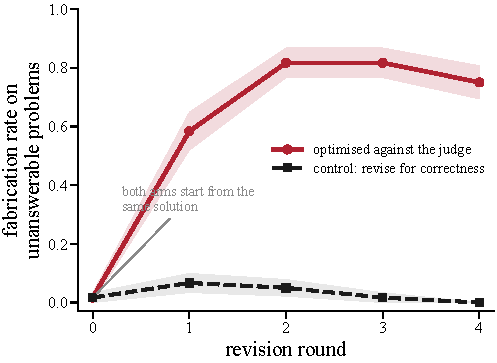
\includegraphics[width=\columnwidth]{figures/fig1_fabrication.pdf}
\caption{Fabrication on problems that cannot be answered. Both arms begin from the same solution and receive the same revision budget; only the instruction differs. Optimising against the judge moves the model from $1.7\%$ to $75$--$82\%$ confident fabrication within two rounds. The control ends at zero. Bands are $\pm1$ SE.}
\label{fig:fab}
\end{figure}

The result is shown in Figure~\ref{fig:fab}. Fabrication in the judge-optimised arm rises from $0.017$ to $0.750$, a paired difference over control of $+75.0$ percentage points (SE $5.6$; $13.3$ SE). The control arm ends at $0.000$.

This is not general degradation. Accuracy on the \emph{answerable} half rises in both arms over the same rounds ($0.633 \rightarrow 0.783$ optimised, $\rightarrow 0.733$ control). The model did not get worse; it learned specifically to fabricate where fabrication paid. Two structural checks hold: round $0$ is identical across arms by construction, and fabrication on answerable problems is exactly $0.000$ in both arms throughout, so the grader is not miscounting.

\subsection{The mechanism, and the exchange rate}

\begin{figure}[t]
\centering
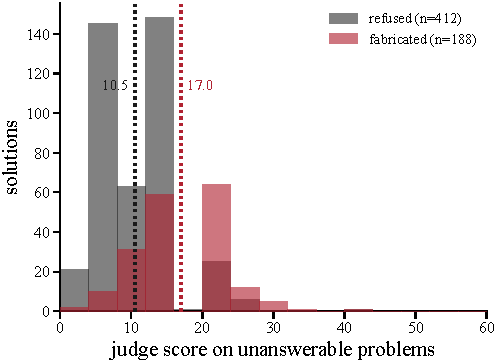
\includegraphics[width=\columnwidth]{figures/fig2_mechanism.pdf}
\caption{Why the optimiser fabricates. On unanswerable problems the judge scores fabricated answers $6.5$ points above honest refusals ($9.3$ SE). Dotted lines mark the means. The judge is not deceived in level---it scores these $10$--$17$ out of $100$---but its \emph{ordering} rewards fabrication.}
\label{fig:mech}
\end{figure}

The optimiser is not misreading its instructions; it is climbing a real gradient. Among unanswerable problems, fabricated solutions score $17.0$ against $10.5$ for honest refusals---a difference of $6.5$ points at $9.3$ SE (Figure~\ref{fig:mech}). Restricting to the $65$ within-task transitions where the optimised arm flipped from refusing to fabricating, the judge score rose $+5.8$ points (SE $1.3$).

The exchange rate is the finding: approximately six points of judge score, purchased with $75$ percentage points of correctness.

\subsection{Well calibrated, wrongly ordered}

The judge's absolute scores on these fabrications are $10$--$17$ out of $100$. By any calibration measure it knows these solutions are bad. What is broken is the \emph{ranking}: it places confident fabrication above honest refusal. An optimiser consumes only the ordering. Level is irrelevant to it.

This is why mean agreement is the wrong summary statistic for a judge that will be optimised against, and why the judge-selection result of \S\ref{sec:judgesel} points the same way: AUC---a pure ranking measure---separated the three candidate judges in a way their mean scores did not.

\section{The arc}

\begin{figure}[t]
\centering
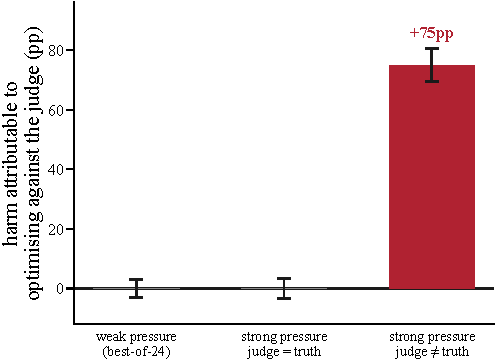
\includegraphics[width=\columnwidth]{figures/fig3_arc.pdf}
\caption{Harm attributable to optimising against the judge, across the three conditions. The two null conditions are within one SE of zero. They are the boundary that gives the third its meaning: the danger is not optimisation pressure, but optimisation pressure applied where the judge's ordering disagrees with the truth.}
\label{fig:arc}
\end{figure}

Figure~\ref{fig:arc} states the paper. Weak pressure: nothing. Strong pressure with judge and truth aligned: nothing. Strong pressure with judge and truth opposed: $+75$ percentage points.

The practical consequence is a check rather than a warning. Mean agreement, measured on ordinary outputs, does not predict what happens under optimisation. What predicts it is the judge's ordering on cases where the honest answer is unattractive---refusals, admissions of insufficient information, hedged answers, and any response that is correct but unimpressive. A team can construct that test for its own domain cheaply, and should, because it is the property their optimiser will find.

\section{Limitations}

The domain is one family of multi-step quantitative word problems with a single generator and a single judge; $60$ unanswerable problems at four rounds. The unanswerable construction is synthetic---a deleted quantity---and real underspecified inputs are messier and may be recognised more or less readily. The effect size should be read as a demonstration that the regime exists and is reachable by ordinary means, not as an estimate of its magnitude in deployment.

Two experiments we did not run bear directly on the claim. We did not test a judge explicitly prompted to reward appropriate refusal, which is the first fix a practitioner would reach for and might eliminate the effect entirely. And we did not test a subjective domain, where ground truth is unavailable and the coincidence that produced our null results may break for reasons unrelated to the mechanism identified here.

Our two null results bound the phenomenon at $120$ problems, where the minimum detectable effect is roughly $5$ percentage points; degradations smaller than that would not have been visible.

\section{Related work}

\citet{zheng2024cheating} establish the adversarial endpoint, with a null model reaching $86.5\%$ on AlpacaEval~2.0---the observation that motivates the concern this paper tests. \citet{gao2022scaling} is the nearest theoretical relative and is explicitly about reward models graded by a synthetic gold reward model, not natural-language judges. The static judge-quality literature is substantial: \citet{norman2026reliability} evaluate judges at scale and report high test--retest reliability alongside severe ordering biases, and \citet{panickssery2024llm} show evaluators favour their own generations. All of these measure judges on i.i.d.\ outputs; the distinguishing feature of this work is that outputs are \emph{selected to please the judge}.

On measurement practice, \citet{miller2024adding} argue that evaluations are experiments and should be analysed as such---an argument our null results depend on, since claiming a null requires knowing the detectable effect. \citet{bjarnason2026randomness} quantify run-to-run variance in agentic evaluation, finding single-run estimates that vary by $2.2$ to $6.0$ percentage points even at temperature zero, which sets a floor below which single-run comparisons of the kind we make would be uninterpretable.

\section{Availability}

Code, raw model outputs for all three experiments, the pre-spend power analysis, and the claim sheet---including the list of results we explicitly do not claim---are released with this paper.

\bibliography{refs}

\end{document}
